\subsection{Loss System}
The Generalized Intersection over Union, an improvement on the traditional Intersection over Union performance metric would be used to more accurately measure the accuracy of the bounding boxes. The GIoU is defined as follows:

\begin{equation}
	GIoU = IoU + \frac{area(B_{GT} \cup B_{PT}}{area(B_{EC}} - 1
\label{eq:GIoU}
\end{equation}

With IoU being defined in Equation~\ref{eq:iou}

\begin{equation}\label{eq:iou}
	IoU = \frac{area(B_{GT} \cap B_{PT}}{area(B_{GT} \cup B_{PT}}
\end{equation}

In those equations, $B_{GT}$ represents the bounding box ground truth, $B_{PT}$ represents the predicted bounding box and $B_{EC}$ represents the smallest enclosing box of $B_{GT}$ and $B_{PT}$.

The GIoU loss is a better measure of the quality of the predicted bounding box. Qian \textit{et al.} also presents a new loss system that has a stronger gradient when the predicted bounding box is farther away to the truth. This loss system is shown in Equation~\ref{eq:giouLoss}

\begin{equation}\label{eq:giouLoss}
	L_{GIoU} = 2 \times log_2 - 2 \times log(1 + GIoU)
\end{equation}

In a recent paper by Ishida \textit{et al.}\cite{ishida2020}, a new kind of regularization is presented, where \textbf{the model is prevented from reaching a zero training loss, even though it has zero training error}. This technique, called \textit{flooding} intentionally prevents further reduction of he training loss when it reaches a certain low value: the \textit{flooding level}. This approach makes the loss move around the flooding level by doing gradient descent if the loss is above the flooding level, but gradient ascent if it is below. This technique allows the network to obtain better generalization results and is very easily implementable.

\begin{figure}[H]
	\begin{subfigure}[t]{.24\textwidth}
  \centering
  % include first image
  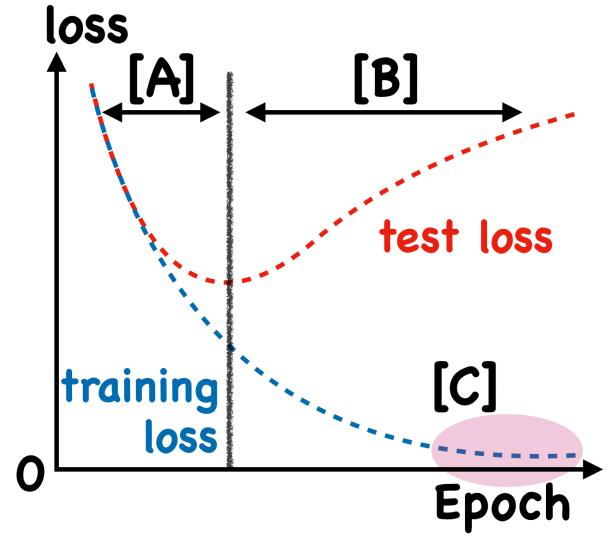
\includegraphics[width=\linewidth]{noLossA}  
  \caption{Without Flooding}
  \label{fig:lossA}
\end{subfigure}
	\begin{subfigure}[t]{.24\textwidth}
  \centering
  % include second image
  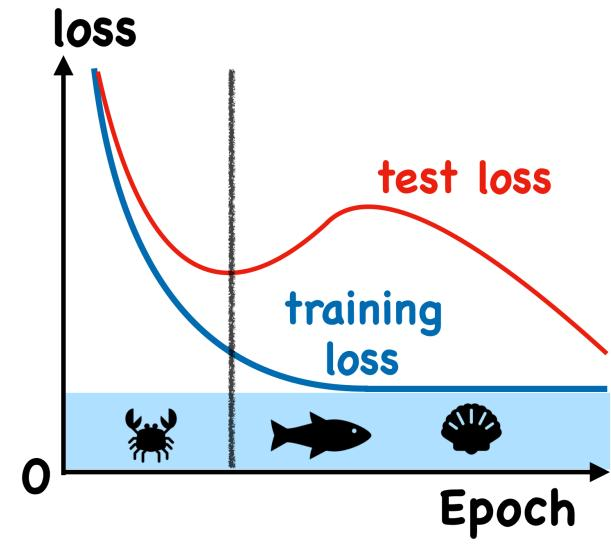
\includegraphics[width=\linewidth]{noLossB}  
  \caption{With Flooding}
  \label{fig:lossB}
\end{subfigure}
	\begin{subfigure}[t]{.24\textwidth}
  \centering
  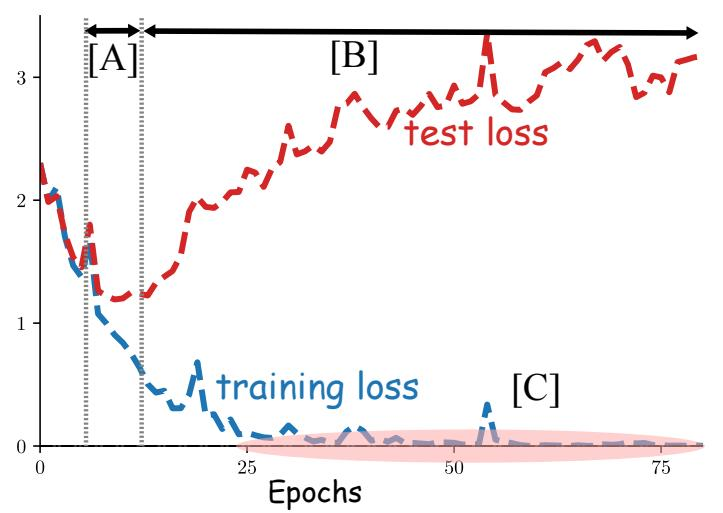
\includegraphics[width=\linewidth]{noLossC}  
  \caption{CIFAR-10 without flooding}
  \label{fig:lossC}
\end{subfigure}
	\begin{subfigure}[t]{.24\textwidth}
  \centering
  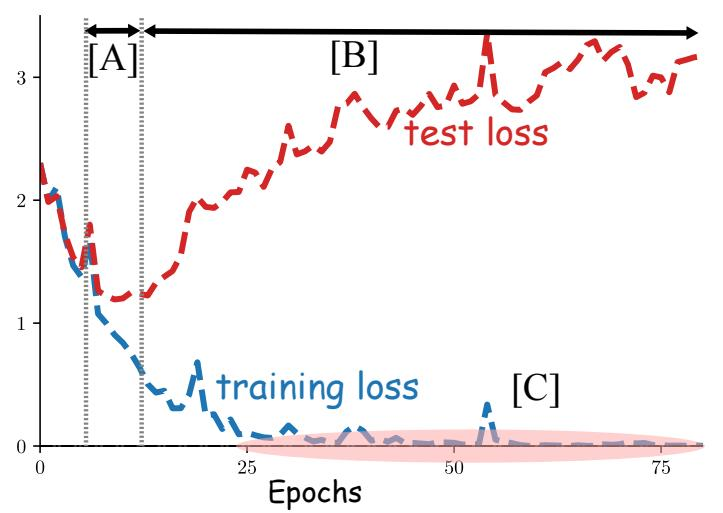
\includegraphics[width=\linewidth]{noLossC}  
  \caption{CIFAR-10 with flooding}
  \label{fig:lossD}
\end{subfigure}
	\caption{Subfigure (a) shows the different regime during which a network first learns, then overfit. During [A], the network learns correctly, and both the training loss and the test loss decreases. During [B] the training loss continues to decreases, but the test loss increases; this is overfitting. In [C] the training loss is nearly zero. The authors show a way to avoid [C] by flooding the bottom area, forcing the loss to stay around a constant, which leads to a decreasing test loss. This is seen in (b) and (c) on the CIFAR-10 dataset}
\label{fig:}
\end{figure}

By letting the loss constant, the model hopefully drift towards a subspace where the loss landscape is flat, leading to better generalization. The authors tested this approach with various datasets, namely MNIST\cite{mnist}, Fashion-MNIST\cite{fashionMNIST}, CIFAR-10\cite{cifar} and often obtained better results and in nearly every datasets, suggesting this approach is effective. Considering the ease of implementation, the lack of performance degradation and the possible improvements on performance, this technique could be very worthwhile.

Finally, in the YOLOv4\cite{yolov4} paper, the author mention the use of \textbf{self adversarial training}. In this training regime, the network first tries to alter the original image instead of its weights. This is an adversarial attack on itself, modifying the original image to fool itself into a wrong inference. Then, the network is trained to detect an object on this modified image in the normal way.

